% v6_draft.tex — Ceremonial Entheogen Use in Puerto Rico
% Phase 5, round 3 (peer review). LaTeX rendering of drafts/v6_draft.md, which is
% v5_draft_human_reviewed.md (Julián + Jean's manual revision of v4) plus this round's
% four review comments. See manuscript/PEER_REVIEW_R3.md for the item-by-item disposition.
%
% Author order, affiliations, Introduction, Methods structure, and Author contributions
% follow the human-reviewed v5, not v4.
%
% Numbers regenerated this round from analysis/missingness.py, analysis/quality.py, and
% analysis/data_prep.load(); the participant-routed base is 67 (not 69) — see the
% comment above Table 2.
% Formatting per manuscript/JOURNAL_REQUIREMENTS.md (Journal of Psychoactive Drugs).
% Word budget: Introduction-Methods-Results-Discussion <= 4,000 words (strict).

\documentclass[12pt]{article}

\usepackage[utf8]{inputenc}
\usepackage[T1]{fontenc}
\usepackage{times}
\usepackage[margin=1in]{geometry}
\usepackage{setspace}
\doublespacing
\usepackage{lineno}
\usepackage{graphicx}
\usepackage{booktabs}
\usepackage{longtable}
\usepackage{amsmath}
\usepackage{url}
\urlstyle{same}  % render URLs in the body font; avoids a Courier dependency
\emergencystretch=3em
\usepackage[authoryear,round]{natbib}
\bibliographystyle{chicago}

\title{Ceremonial Entheogen Use in Puerto Rico: A Descriptive Survey of Participants
and a Small Facilitator Subsample}

\author{
  Jean C. V\'elez Rodr\'iguez$^{1}$ \and Juli\'an M. Hern\'andez Torres$^{1,2}$ \and
  Ang\'elica N. Grajales Rold\'an$^{1,8}$ \and Juliana Mill\'an-Torres$^{3}$ \and
  Paulina D. Rull\'an Farinacci$^{4,5,6}$ \and Adriana I. Rodr\'iguez Massa$^{7}$ \and
  Carolina Riollano$^{3}$ \and Yamil O. Ortiz Ortiz$^{8}$ \\[1em]
  \begin{minipage}{0.92\textwidth}\centering\small\setstretch{1.15}
  $^{1}$Puerto Rico Institute for Psychedelic Science, Medicine \& Awareness, San Juan, Puerto Rico \\
  $^{2}$Behavioral Sciences Research Institute, University of Puerto Rico, Medical Sciences Campus,
  San Juan, Puerto Rico \\
  $^{3}$Red Enteog\'enica de Puerto Rico, Colectivo Psicod\'elico de Puerto Rico and Within Psychological
  Services, San Juan, Puerto Rico \\
  $^{4}$Department of Psychiatry, School of Medicine, University of Puerto Rico, Medical Sciences Campus,
  San Juan, Puerto Rico \\
  $^{5}$Pravan Foundation \\
  $^{6}$Sattva Clinic \\
  $^{7}$Department of Psychology, University of Puerto Rico, R\'io Piedras Campus, San Juan, Puerto Rico \\
  $^{8}$Centro de Investigaciones Sociales, Facultad de Ciencias Sociales, University of Puerto Rico,
  R\'io Piedras Campus, San Juan, Puerto Rico \\[0.5em]
  Corresponding author: Jean C. V\'elez Rodr\'iguez, jean.velez5@upr.edu
  \end{minipage}
}

\date{}

\begin{document}

\maketitle
\linenumbers

\begin{abstract}
\noindent
% ABSTRACT — unstructured, <=200 words (JPD requirement).
Ceremonial entheogen use occurs in Puerto Rico outside clinical and regulatory structures, and the
practices surrounding it have not been described. We conducted an anonymous, bilingual, cross-sectional
online survey of adults aged 21 and over reporting involvement in entheogen-assisted ceremonies in Puerto
Rico, recruited by convenience and chain referral, February--June 2026. Of 100 submissions, 73
identified a role: 72 as participants and 8 as facilitators, 7 of whom were both. Respondents were
middle-aged (mean 42.4 years), mostly university-educated, and almost all resident in Puerto Rico. Most
recent ceremonies were typically single, multi-hour events in natural settings involving psilocybin
mushrooms or ayahuasca, and satisfaction was strongly ceiling-weighted (median 6 of 6). Preparation was
near-universal among those answering while pre-ceremony screening was not, and the small facilitator
subsample described training and emergency planning as informal rather than credentialed. Five of 67
participants answering reported ever experiencing non-consensual physical contact during a ceremony, and 2
of 65 at their most recent one. A comparison of any preparation against none, specified in the analysis
plan before testing, was positive in direction but rests on five unprepared respondents and is exploratory.
These findings describe this sample only and support no prevalence or causal claim.
\end{abstract}

\noindent\textbf{Keywords:} entheogens; psychedelics; ceremonial use; Puerto Rico; harm reduction; survey research

\section{Introduction}

Ceremonial use of entheogens, psilocybin-containing mushrooms, ayahuasca, and related preparations taken
in structured group or guided settings, has become substantially more visible across the Americas over the
past two decades, largely outside the clinical-trial infrastructure that generates most of the contemporary
research literature \citep{carvalho2025scoping}. The resulting evidence base is asymmetric. Randomized
clinical trials characterize carefully screened participants receiving standardized doses under monitored
conditions, and its samples remain ethnoracially narrow
\citep{hughes2024ethnoracial,marcus2026psychedelics}. On the other hand, community ceremonial practice is
documented mainly through ethnographic and qualitative work, with comparatively few survey-level
descriptions of who takes part and under what conditions
\citep{carvalho2025scoping,teixeira2026ayahuasca}.

Puerto Rico occupies an unusual position as a Spanish-speaking Caribbean jurisdiction where psilocybin,
N,N-dimethyltryptamine (DMT), and related compounds remain Schedule I under the federal Controlled Substances Act
\citep{uscongress1970csa} and the territory's aligned statute \citep{pr1971csa}, outside the
decriminalization and regulated-access reforms reshaping parts of the United States
\citep{siegel2023psychedelic}. It is also a setting with a long-documented tradition of spiritually framed
healing practice (i.e.\ espiritismo and related practices) described in the clinical and public health
literature for more than four decades
\citep{koss1980therapist,comasdiaz1981puertorican,bird1981sociopsychiatry,zerrate2022espiritismo}.

Local survey evidence on entheogen use is nonetheless minimal. To the authors' knowledge, only one
published Puerto Rico--specific survey exists \citep{velezrodriguez2026psilocybin}. This survey
characterized psilocybin use patterns, motivations, and personality correlates. Another survey, as part of
an unpublished thesis, examined perceptions of psilocybin mushrooms in a non-random sample of university
students \citep{doeltermorales2020hongos}. However, neither study collected data on ceremonial entheogen
use patterns, outcomes, practices, and safety. In addition, both studies focused mainly on psilocybin use
without expanding on other substance use patterns, and neither describes how ceremonies are conducted. No
descriptive characterization of ceremonial use of entheogens in Puerto Rico currently exists.

A descriptive characterization can contribute to an evidence base on ceremonial entheogen use in Puerto
Rico in three ways. First, it establishes whether practices reported here resemble a harm-reduction
approach. Harm-reduction considerations include but are not limited to: preparation, screening,
environment, ethical and legal issues, managing emergencies or difficult experiences, and integration of
the experience \citep{gorman2021psychedelic,pilecki2021ethical,dutton2025harm}. Second, it provides initial
data on safety outcomes and adverse experiences, such as inappropriate sexual contact and sexual abuse,
within these communities in Puerto Rico \citep{kruger2025psychedelic,peluso2020reflections}. Third, it
produces instrument-level evidence that provides insights into future research directions and the necessity
of higher-powered studies.

This study aims to describe a sample of participants and facilitators of ceremonial entheogen use in Puerto
Rico, and to examine bivariate associations between preparation and reported ceremony outcomes and between
participant-reported facilitator practices and perceived safety.

\section{Methods}

\subsection{Design, ethics, and consent}

This study employed a cross-sectional, self-administered, non-probability online survey design. We collected
data on a sample of adults 21 and older reporting prior involvement in entheogen-assisted spiritual
ceremonies in Puerto Rico using a self-administered questionnaire fielded on KoboToolbox
\citep{kobotoolbox2026} between 24 February and 9 June 2026. Participation was fully anonymous: no names,
dates of birth, or other personal identifiers were collected. The information sheet (purpose, procedures,
risks, voluntariness, data retention) was presented within the questionnaire itself. Respondents who read it
and proceeded thereby gave informed consent. No signed consent document was collected or required. Every
item offered a ``prefer not to answer'' option and withdrawal was permitted at any point. No compensation
was offered, and mental-health resources were listed for the participants' benefit. Reporting follows STROBE. The study was approved by the Institutional Review Board of
the University of Puerto Rico, Medical Sciences Campus (OPPHIE 2509472552).

\subsection{Recruitment and sample construction}

Recruitment used convenience sampling with chain referral, promoted through Facebook, Instagram, Twitter/X,
and WhatsApp and by bulletin-board announcements at the University of Puerto Rico R\'io Piedras and Medical
Sciences campuses. Inclusion criteria were age 21 or older, ability to read and write in Spanish, access to
an internet-connected device, and prior participation in an entheogen-assisted spiritual ceremony in Puerto
Rico.

Sample construction is shown in Figure~\ref{fig:flow}. Out of 100 submissions, 13 were abandoned and 14 of
the remaining 87 screened out (16\%), leaving the analytic sample of $N=73$. Seven of the 8 facilitators
also identified as participants.

\subsection{Instrument}

To the authors' knowledge, no validated Spanish-language instrument for characterizing ceremonial entheogen
use exists for Puerto Rico, so the questionnaire was purpose-built by the research team, whose members had
direct experience with ceremonial psychedelic/entheogen practice in Puerto Rico and used that experience to
inform item content. Development proceeded in stages: an initial list of target constructs was drawn from
the study's research questions and hypotheses; a pool of candidate items was drafted from that list; items
were then reviewed iteratively by the full team to correct errors, consolidate and adjust response
categories, and revise wording for clarity and relevance; and items judged out of scope, irrelevant, or too
sensitive for the study's objectives were removed. The retained item set was translated from Spanish to
English by a professional translator using a direct-translation technique, after which the team performed a
final bilingual pass to check grammatical accuracy and equivalence between language versions.

No formal pretesting (cognitive interviewing, expert content-validity review, or a pilot administration)
preceded fielding, and no back-translation was performed. The present analysis therefore constitutes the
first reliability evidence for the instrument rather than a validation of an existing one. The questionnaire
was administered as an anonymous, self-administered online survey (KoboToolbox XLSForm), with branching skip
logic gating sociodemographic and role-specific items behind an eligibility/consent screen and a subsequent
role self-identification item. Nearly every item offered a ``prefer not to answer'' option. Seven
attention-check items were included, administered separately by branch (three for facilitators, four for
participants) rather than uniformly across the full sample. Completion was estimated at 20--25 minutes.
Verbatim English wording and response anchors for the items carrying the principal results appear in
Table~\ref{tab:items}. Because both language versions live in one form rather than in two parallel
questionnaires, every respondent saw the same item set regardless of the language they answered in.

\subsection{Measurement}

The primary outcome, satisfaction with the most recent ceremony, was a 0 (very unpleasant)--6 (very
pleasant) ordinal item. The primary exposure captured self-directed preparation for these ceremonies, aside
from facilitator instructions (yes/sometimes/no). The two differ in referent: the outcome asks about one
event, the exposure about a general practice. Secondary participant-side measures (comfort and safety,
trust in the facilitator, prior knowledge of the facilitator's background, screening questions asked, and
prior disclosure to a health professional) all refer to the most recent ceremony. The non-consensual contact
item asked whether the respondent had \emph{ever} experienced unexpected or unclearly consented physical
touch during a ceremony, explicitly including moments of uncertainty or absent recall. A parallel
most-recent-ceremony item is also reported. Facilitator-branch items covered training, screening approach,
distress-response protocol, emergency planning, and crisis signs witnessed. Three substance variables were
kept distinct and never merged: facilitator-led, participant (all ceremonies attended), and
most-recent-ceremony. Attention checks were branch-specific.

\subsection{Missing data and data quality}

Missingness was decomposed per item into four mutually exclusive states: answered substantively, answered
``prefer not to answer'' or ``not sure'', left blank while routed, and never shown by the skip
logic (Table~\ref{tab:missingness}). Almost all apparent missingness on the participant items is structural:
5 of the 72 participant-side respondents were never routed to the participant section, and among the 67 who
were, genuine item nonresponse never exceeded 3 respondents (4.5\%) on any item, the maximum falling on the
satisfaction outcome. Retained non-response categories were more common than blanks and concentrated on a
single item, whether the facilitator asked screening questions (12 of the 67 answering ``not sure'' or
``prefer not to answer''). On the facilitator side each item was left blank by 1 of the 8 routed
respondents. No imputation was performed, and no item approached a level of nonresponse at which it would be
warranted.

Attention checks were branch-specific rather than uniform so each respondent was judged only on their own branch. Facilitators answered 21 of 21
attention items correctly; participants answered 241, of which 3 were incorrect, concentrated in 2
respondents. Per protocol both were flagged and retained, not dropped. Because the platform never populated
its duplicate-detection field and recorded no IP or device information, duplicate submissions were screened
manually on the respondent-chosen nickname and password. Exactly one exact nickname-and-password match
exists across the 100 submissions, and its earlier member is a blank abandoned submission already excluded
before analysis; nickname-only and password-only repeats were common Spanish words that respondents in this
thematic context would plausibly choose independently. No analytic row required exclusion on duplicate
grounds.

\subsection{Statistical approach}

The outcome distribution was strongly ceiling-weighted and several exposures had thin or unbalanced
categories, so all tests were nonparametric: Mann--Whitney $U$, Kruskal--Wallis $H$, permutation $\chi^2$
with 10,000 label permutations (seed 20260715) for thin contingency tables, and Fisher's exact test at very
small $n$. Effect sizes were rank-biserial $r_{rb}$ with the common-language effect size, epsilon-squared
$\varepsilon^2$, and Cram\'er's $V$ respectively, with Wilson 95\% confidence intervals for prevalences.

The preparation-to-satisfaction comparison was designated in the analysis plan as the primary comparison
before any test was run, and is reported uncorrected, with a tie-aware permutation test as a robustness
check because the outcome is heavily tied. All other bivariate tests were assigned to four prespecified,
thematically organized families, such as bivariate, substance-stratified, safety-domain, and legal-knowledge,each
corrected jointly by the Benjamini--Hochberg procedure. Analyses were conducted
in Python; the full pipeline is available (see Data availability).

\subsection{Protocol deviations}

Three deviations are reported transparently. The protocol's preparation $\times$ integration design
is not estimable: the instrument has no clean participant integration-received item, and the preparation
split is badly unbalanced, so preparation was examined against the outcome directly and no integration
measure is reconstructed anywhere. The protocol also specified crossing facilitator training and protocol
items against participant-perceived safety; since facilitator self-report cannot be linked to the ceremony
any participant attended, these would have paired unrelated events. Two participant-answerable proxies
substitute for the first (prior knowledge of the facilitator's background and whether screening questions
were asked) facilitator self-report is presented separately and descriptively, and a facilitator-side
readiness composite replaces the mixed one. Two skip-logic errors in the instrument were also identified
and are described in the Limitations.

\section{Results}

\subsection{Respondents}

The analytic sample of 73 adults skewed middle-aged and highly educated (Table~\ref{tab:demo}) with mean age
42.4 years, 49\% women, 78\% holding a bachelor's degree or above, and 61\% describing their economic
situation as comfortable. Sixty-eight (94\% of the 72 answering) reported residing in Puerto Rico. Free-text
engagement was substantial relative to sample size: 37 open-text fields yielded 285 non-empty answers,
roughly three-quarters in Spanish.

\subsection{The ceremonial context}

Participants reported extensive but not recent ceremonial histories. Among the 67 answering, the median
number of lifetime ceremonies attended was 6 (IQR 3--12, range 1--250) against a median of 1 in the past 12
months (IQR 0--2), and 45\% reported their last ceremony more than 12 months earlier
(Table~\ref{tab:context}).

Across all ceremonies attended, participants most often reported magic mushrooms, ayahuasca, tobacco, and
cacao, followed by an ``other'' category that only 3 of the 18 selecting it specified via free text, and
then DMT, lysergic acid diethylamide (LSD), 3,4-methylenedioxymethamphetamine (MDMA), and ketamine, in
descending order (Figure~\ref{fig:subs}, base $n=67$). For the most
recent ceremony, the individually reportable groups were magic mushrooms ($n=31$) and ayahuasca ($n=23$),
every remaining substance being pooled into a combined group ($n=11$) under a prespecified rule.

The most recent ceremony was typically a discrete, multi-hour, outdoor event: a single ceremony rather than
a retreat for 74\%, a natural setting for 55\%, and most often either 4--6 hours or an overnight event of
roughly 12 hours or more (Table~\ref{tab:context}).

\subsection{Preparation, screening, and prior knowledge}

Preparation was near-universal among those answering: 82\% prepared and 9\% sometimes did, against 9\%
reporting none (Table~\ref{tab:safety}). Participant-observable facilitator practices were common but not
uniform as 81\% knew about the facilitator's background beforehand, but only 59\% reported being asked
screening questions, against 23\% who were not and 11\% who were unsure. Disclosure outside the ceremonial
context was uncommon: 12\% had spoken to a health professional about their participation beforehand.
Among the 54 respondents who answered all three of preparation, prior knowledge of the
facilitator's background, and screening, every one reported at least one of them.

\subsection{Experience and perceived safety}

Reported satisfaction was overwhelmingly positive and strongly ceiling-weighted: 63 of the 72 participants
gave a numeric score, with a median of 6 and the mode at the scale maximum (Figure~\ref{fig:good}'s caption
decomposes the remainder into structural skips, item nonresponse, and a ``prefer not to answer'').
Perceived in-ceremony comfort and safety was similarly high and undifferentiated, returning a median of 3 in
both facilitator-background subgroups large enough to characterize ($n=54$, $n=8$; the third, $n=2$, is not)
and differing neither by that background knowledge nor by whether screening questions were asked. Trust in
the facilitator was the one participant-side comparison differing at the uncorrected level: median 4 (IQR
3--4) among the 54 who knew the facilitator's background beforehand against 3 among both smaller groups
($H=8.15$, $p=0.017$, tie-aware permutation $p=0.010$, $\varepsilon^2=0.10$; thinnest group $n=3$), and did
not survive correction ($q=0.085$). Satisfaction did not differ significantly by most-recent-ceremony
substance ($H=4.98$, $p=0.083$, $q=0.166$).

Of the 67 participants answering the lifetime non-consensual contact item, 61 (91\%) reported no such
contact, 5 (7\%) reported that it occurred, and 1 was unsure; the within-sample proportion was 7.5\% (Wilson
95\% CI 3.2--16.3). The parallel most-recent-ceremony item, answered by 65, returned 2 affirmative and 62
negative, with 1 declining: of the 5 reporting the experience ever, 2 placed it at the most recent ceremony
and 3 did not. Non-consensual contact was associated with prior knowledge of the facilitator's background at
the uncorrected level (permutation $\chi^2=18.90$, $p=0.047$, $V=0.38$, $n=67$) but not with screening
(permutation $\chi^2=13.64$, $p=0.094$, $V=0.32$, $n=66$); neither survived correction (both $q=0.188$), nor
did the comparison by substance ($p=0.486$).

\subsection{Facilitator practice}

Eight respondents identified as facilitators, 7 of whom also identified as participants; the eighth, the
sole facilitator-only respondent, answered no facilitator item, so every proportion below is of the 7 who
answered. Preparation for the role came from personal experience and self-study (6 of 7), mentorship or
apprenticeship (4), and family or ancestral tradition (3); \emph{none} reported formal certification or
academic coursework. Screening was conversational rather than structured: 6 began with an interview or
conversation, 4 asked about medical history and 4 about current medication, 3 asked about mental-health
challenges, and 2 said they welcome anyone who feels called to take part. Responses to a difficult
experience were likewise non-clinical --- singing, music, or sound (5), grounding exercises (4), calming
words (3), consented physical touch (2), with one reporting use of a ``trip killer'' medication and one
never having faced the situation. Six gave preparation instructions beforehand and six worked outdoors or
near nature. Dosing was mostly devolved to participants (3 of 7). Emergency planning was informal or
unwritten (4) or dependent on the situation (3), and \emph{none} selected a formal written plan.

All 7 reported witnessing crisis signs, most commonly disorientation, feeling overwhelmed, fainting,
difficulty breathing, or panic attacks (each $n=3$), and less often signs of self-harm or suicidal thoughts
($n=2$). These counts are not rates: three respondents reported several signs each, two reported a single
sign, one answered only ``I'm not sure'' and one only ``other'', so the distribution concentrates in three
people. Association tests within this branch returned undefined odds ratios, Fisher's exact
$p=0.143$ against the distress-response protocol and $p=0.429$ against the emergency plan, with two further
tests unrunnable for want of non-degenerate data; every $2\times2$ table here has at least one margin of two
or fewer. They establish an analytic approach for a larger facilitator sample rather than evidence for or
against any association.

\subsection{Preparation and reported satisfaction}

Among the 63 participants, 58 reported some preparation (median 6, IQR 5--6) and 5 reported none (median 4,
IQR 3--5; Figure~\ref{fig:prep}); a sixth respondent reporting no preparation did not answer the outcome,
which is why this base is 5 rather than the 6 in Table~\ref{tab:safety}. A Mann--Whitney comparison returned
$U=218.0$, $p=0.041$, $r_{rb}=0.50$, and a common-language effect size of 0.75; a tie-aware permutation test
gave $p=0.024$.

\section{Discussion}

\subsection{A structurally informal practice landscape}

The most stable picture this sample supports is a practice organized around informal, relationally
transmitted expertise rather than credentialed or documented protocol. Among the facilitators who
self-reported, training came from personal experience, self-study, mentorship, and family tradition; none
reported formal certification or academic coursework, and emergency planning was uniformly informal or
conditional. This sits at some distance from the structured preparation, screening, and difficult-experience
protocols that harm-reduction frameworks for psychedelic settings assume \citep{dutton2025harm}, is
consistent with survey evidence that people who use psychedelics support clearer practice standards
\citep{kruger2023preferences}, and is a reminder that in community settings the containing structure is the
setting itself rather than a protocol \citep{hartogsohn2017constructing}.

On the participant side the informality reads differently. Preparation was near-universal among those
answering, but roughly a quarter reported that no screening questions were asked and a further group was
uncertain. The asymmetry is worth separating: preparation is something participants largely do, whether
self-directed or instructed, whereas screening must be done \emph{to} them, and was substantially less
consistent here. If that asymmetry holds in a larger sample it would locate the intervention target on the
facilitator side, which this sample cannot establish.

The demographic profile, middle-aged, university-educated, economically comfortable, resembles
ceremony-attender cohorts described elsewhere, though older and more educated. Its mean age of 42.4 years
and 78\% holding a bachelor's degree or above compare with 37.6 years and 49\% degree-holding among North
America neo-shamanic ayahuasca ceremony attenders \citep{pagni2025longterm}, 37.0 years among ceremonial
ayahuasca retreat attenders in the Peruvian Amazon \citep{ruffell2021ceremonial}, and 40 years with 59\%
degree-holding in a large international naturalistic psilocybin cohort \citep{nayak2023naturalistic}; the
49\% here identifying as women falls inside the 44--61\% those three report, as it does for international
psychedelic-survey samples \citep{kopra2023investigation,robinson2026field} and the
psilocybin-specific Puerto Rico survey \citep{velezrodriguez2026psilocybin}. That convergence is best read
as evidence about who responds to online psychedelic surveys, not about who attends ceremonies
\citep{bethlehem2010selection}.

\subsection{A ceiling that limits what satisfaction can reveal}

Reported satisfaction clustered at the top of its scale, and a perceived-life-impact item had no variance at
all, a substantive finding, consistent with naturalistic cohorts reporting predominantly positive appraisals
\citep{nayak2023naturalistic,ruffell2021ceremonial}, but one that also constrains the analysis severely. An
outcome with almost no variance in the lower range cannot discriminate between groups, and the null results
across the corrected families are consistent with that constraint rather than with the absence of any
association. Ceiling behavior is a known property of self-report scales for hallucinogen experience rather
than a peculiarity of this instrument \citep{bouso2016measuring}. Satisfaction, measured this way, is close
to exhausted as an outcome here; future work needs measures with headroom in both directions before group
comparisons on experience quality can be informative.

\subsection{Safety signals the design can identify but not quantify}

Five of 67 participants answering reported non-consensual physical contact at some point, two of them at
their most recent ceremony, and facilitators reported having witnessed crisis signs at a base of seven at
which no rate is estimable. These come from different reporters and cannot be combined. That such reports
appear at all is consistent with survey-based evidence on boundary violations in naturalistic psychedelic
settings \citep{kruger2025psychedelic,mcnamee2023studying} and with the community harm-reduction literature
that developed in response \citep{peluso2020reflections}, and the crisis signs described are of a kind
documented at non-trivial rates in large naturalistic samples
\citep{carbonaro2016survey,bouso2022adverse}. The item used here was deliberately broad, covering
unexpected touch and uncertain or unremembered consent, so the figure should not be read against a narrower
legal or clinical standard.

The study establishes that these events occur among respondents and that an instrument of this kind can
capture them; it cannot establish how often they occur, in whom, or under what conditions. The
cross-tabulations against participant-side proxies are powered neither to confirm nor to rule out an
association and did not survive correction, so treating any of them as an actionable signal would overstate
them considerably. The safety domain justified its inclusion by identifying a measurement priority, not by
producing an estimate.

\subsection{Limitations}

The sample was non-probability, unweighted, and self-selected; the concentration in higher education and
favorable economic self-ratings describe who responded, not who participates, and nothing here supports a
statement about how common ceremonial entheogen use is in Puerto Rico. Roughly 6\% of those answering the
residency item lived outside Puerto Rico, further tempering a Puerto Rico--specific reading, and eligibility
criteria were self-assessed rather than enforced.

Role subsamples were small and unevenly sized, and the facilitator branch of eight supports no rate and no
association test. Because 7 of those 8 also answered as participants, the facilitator-side and
participant-side statistics are not independent samples and should not be read as two separate groups. The
reports are nonetheless unlinked at the ceremony level, which eliminated the protocol's integration-proxy
comparison, its perceived-safety-by-training analysis, and its mixed harm-reduction composite.

The preparation-to-satisfaction comparison is this study's most fragile result. The direction was positive
and the effect sizes were not small, but the no-preparation group contained five respondents answering the
outcome. Nothing here establishes the finding. The preparation split remains the binding constraint on the
primary analysis, so any successor study will need either a sampling strategy that reaches unprepared
participants in usable numbers or a question that does not depend on that contrast.

Two referent mismatches limit the associations reported here. The safety cross-tabulations pair a lifetime
outcome with most-recent-ceremony exposures, so for the 3 respondents who reported non-consensual contact at
some ceremony other than their most recent one, exposure and outcome describe different events. The primary
comparison pairs a most-recent-ceremony outcome with a general-practice exposure.

All measures were single-timepoint self-report, and for most respondents the most recent ceremony was
distant (45\% reported more than 12 months ago) so recall error is plausible and unmeasurable. The
instrument contains no integration measure, is unvalidated, and produced only preliminary two-item
reliability evidence ($\alpha=0.58$ for trust and in-ceremony comfort; $\alpha=0.86$ for the two
legal-knowledge items). Two skip-logic errors were identified in the fielded form and are reported so a
future deployment can correct them. A follow-up item asking why a respondent felt uncomfortable or unsafe
required the comfort-and-safety variable to equal two different values at once, making it structurally
unreachable rather than merely unpopular: no respondent could have answered it. A general legal-worry item
was gated on the general legal-knowledge item equalling ``prefer not to answer'', the opposite of what a
parallel item would require, so only six respondents reached it while its most-recent-ceremony counterpart
was asked broadly ($n=57$); the two are neither comparable nor parallel, and the general item is excluded
from all analyses. Two
response categories are uninterpretable as collected: the substance ``other'' option, specified in free text
by only 3 of the 18 who selected it, and the 12 of 67 respondents answering ``not sure'' or ``prefer not to
answer'' on whether they were screened.

\subsection{Conclusion}

Within this self-selected sample of 73 adults, ceremonial entheogen use in Puerto Rico is described by a
middle-aged, university-educated, overwhelmingly Puerto Rico--resident group whose most recent ceremonies
were typically single, multi-hour, outdoor events described in strongly positive terms. Preparation was
near-universal while screening was not, and the small facilitator subsample described training and
emergency planning as informal. Five of 67 reported non-consensual physical contact, and facilitators
reported crisis events at a base too small to rate. These findings describe this sample alone, support no
prevalence estimate and no inference about what any practice produces, and take their principal value from
identifying what a properly powered successor study would need to measure, sample, and correct.

\section*{Author contributions}
Roles follow the CRediT taxonomy (\textsf{credit.niso.org}).

\noindent\textbf{Jean C. V\'elez Rodr\'iguez:} Conceptualization; Methodology (supporting); Software;
Formal analysis (lead); Data curation; Visualization; Writing --- original draft; Writing --- review \&
editing; Project administration.

\noindent\textbf{Juli\'an M. Hern\'andez Torres:} Conceptualization; Methodology (lead); Validation;
Formal analysis (supporting); Writing --- review \& editing; Project administration.

\noindent\textbf{Ang\'elica N. Grajales Rold\'an:} Methodology (supporting); Investigation; Writing ---
review \& editing.

\noindent\textbf{Juliana Mill\'an-Torres:} Conceptualization; Methodology (supporting); Validation
(supporting); Writing --- review \& editing.

\noindent\textbf{Paulina D. Rull\'an Farinacci:} Conceptualization; Methodology (supporting); Validation
(supporting); Writing --- review \& editing.

\noindent\textbf{Adriana I. Rodr\'iguez Massa:} Methodology (supporting); Investigation; Writing ---
review \& editing.

\noindent\textbf{Carolina Riollano:} Conceptualization; Methodology (supporting); Validation
(supporting); Writing --- review \& editing.

\noindent\textbf{Yamil O. Ortiz Ortiz:} Supervision; Writing --- review \& editing.

\noindent All authors reviewed and approved the final manuscript.

\section*{Funding}
This research received no specific grant from any funding agency in the public, commercial, or
not-for-profit sectors.

\section*{Competing interests}
Several authors are affiliated with organizations that conduct, advocate for, or provide services related
to psychedelic and entheogen research and practice. Affiliation with the Puerto Rico Institute for
Psychedelic Science, Medicine \& Awareness, the Pravan Foundation, and the Colectivo Psicod\'elico de
Puerto Rico is disclosed as a non-financial competing interest. In addition, Juliana Mill\'an-Torres owns
Within Psychological Services and Paulina D. Rull\'an Farinacci serves as Chief Medical Officer of Sattva
Clinic; both are disclosed as financial competing interests. No other author received financial support
from, or holds a financial interest in, any commercial entity with an interest in the subject matter of
this article.

\section*{Data availability}
The anonymous survey data and the complete analysis code that generates every result reported here will
be deposited in a public repository on publication, and the digital object identifier will be recorded
here. The data contain no direct identifiers by design. Until deposit, both are available from the
corresponding author. Every number reported here is generated by an executable Python pipeline that reads
the raw survey export and the XLSForm directly, so all response decodes derive from the form rather than
from hand-entered value maps; the pipeline regenerates the full analysis in one command.

\section*{Generative AI use declaration}
Large language model tooling was used to assist with statistical analysis code development and with
drafting and editing of this manuscript. Specifically, the authors employed Opus 5 and Sonnet 5. All analyses were specified by the authors, all outputs were
verified against the source data by the authors, and the authors take full responsibility for the content
of this article.

\bibliography{../references/references}

\clearpage

\section*{Tables and Figures}

\begin{table}[htbp]
\centering
\small
\setstretch{1.0}
\caption{Verbatim English wording and response anchors for the items carrying the principal results. The
questionnaire was a single bilingual XLSForm with Spanish as the default language and English selectable
through the platform's language switcher: every item carries both labels in the same form, so this is a
native bilingual instrument rather than a post-hoc translation of a Spanish original. Note that the raw
comfort-and-safety option list is stored best-first; the analysis re-orders it so that a higher code always
means a more positive response, consistent with every other ordinal scale here.}
\label{tab:items}
\vspace{0.8em}  % long caption; without this its last line lands on the toprule
\begin{tabular}{p{3cm}p{5.6cm}p{5.4cm}}
\toprule
Item (construct) & Wording & Response options \\
\midrule
Satisfaction \newline (primary outcome) &
``From 0 to 6, how pleasant was the ceremony?'' &
0 Very unpleasant; 1 Unpleasant; 2 Somewhat unpleasant; 3 Neither pleasant nor unpleasant; 4 Somewhat
pleasant; 5 Pleasant; 6 Very pleasant; Prefer not to answer \\
\addlinespace
Self-directed preparation \newline (primary exposure) &
``Aside from the facilitator's instructions or recommendations, do you personally engage in preparation for
these ceremonies?'' &
Yes; Sometimes; No; Prefer not to answer \\
\addlinespace
In-ceremony comfort and safety &
``During the ceremony, how would you describe your overall sense of comfort and safety?'' &
0 I felt very uncomfortable or unsafe; 1 At times I felt somewhat uncomfortable or unsafe; 2 I felt mostly
comfortable and safe; 3 I felt completely comfortable and safe; Prefer not to answer \\
\addlinespace
Trust in facilitator &
``How much did you trust the person who facilitated the ceremony?'' &
0 Not at all; 1 A little; 2 Moderately; 3 A lot; 4 Completely; Prefer not to answer \\
\addlinespace
Non-consensual physical contact \newline (lifetime) &
``Have you ever experienced physical touch during a ceremony that felt unexpected or that you did not
clearly agree to beforehand? This could include moments where you were unsure, uncomfortable, or did not
remember giving permission.'' &
Yes; No; I'm not sure; Prefer not to answer \\
\addlinespace
Non-consensual physical contact \newline (most recent ceremony) &
``During your most recent ceremony, did you experience any physical touch that felt unexpected or that you
didn't clearly agree to beforehand?'' &
Yes; No; I'm not sure; Prefer not to answer \\
\bottomrule
\end{tabular}
\end{table}

\clearpage
\begin{table}[htbp]
\centering
\small
\caption{Missing-data decomposition by item, analytic sample ($N=73$). The four states are mutually exclusive and sum to 73 on every row. \emph{Substantive} = a real response category; \emph{PNA/not sure} = a retained non-response category, kept as its own category throughout and never dropped; \emph{Blank} = routed to the item and left empty, the only genuine item nonresponse; \emph{Not routed} = the skip logic never showed the item. Routing conditions are transcribed from the XLSForm \emph{relevant} expressions, not inferred from empty cells.}
\label{tab:missingness}
\setstretch{1.0}
\begin{tabular}{lrrrr}
\toprule
Item & Substantive & PNA/not sure & Blank & Not routed \\
\midrule
\addlinespace
\multicolumn{5}{l}{\emph{Sociodemographic branch --- routed $n=73$ of 73}} \\
Age & 72 & 0 & 1 & 0 \\
Gender & 71 & 0 & 2 & 0 \\
Education & 72 & 0 & 1 & 0 \\
Economic situation & 70 & 2 & 1 & 0 \\
Country of residence & 72 & 0 & 1 & 0 \\
\addlinespace
\multicolumn{5}{l}{\emph{Participant branch --- routed $n=67$ of 73}} \\
Substances, all ceremonies attended & 67 & 0 & 0 & 6 \\
Substance, most recent ceremony & 65 & 1 & 1 & 6 \\
Time since last ceremony & 65 & 1 & 1 & 6 \\
Place, most recent ceremony & 66 & 1 & 0 & 6 \\
Format, most recent ceremony & 62 & 3 & 2 & 6 \\
Duration, most recent ceremony & 65 & 0 & 2 & 6 \\
Self-directed preparation & 67 & 0 & 0 & 6 \\
Knew facilitator's background & 66 & 1 & 0 & 6 \\
Facilitator asked screening questions & 54 & 12 & 1 & 6 \\
Spoke to a health professional beforehand & 62 & 3 & 2 & 6 \\
Satisfaction, most recent ceremony & 63 & 1 & 3 & 6 \\
Trust in facilitator & 65 & 2 & 0 & 6 \\
In-ceremony comfort and safety & 65 & 1 & 1 & 6 \\
Non-consensual contact, ever & 66 & 1 & 0 & 6 \\
Non-consensual contact, most recent & 64 & 1 & 2 & 6 \\
\addlinespace
\multicolumn{5}{l}{\emph{Facilitator branch --- routed $n=8$ of 73}} \\
Facilitator training background & 7 & 0 & 1 & 65 \\
Emergency plan & 7 & 0 & 1 & 65 \\
Crisis signs witnessed & 6 & 1 & 1 & 65 \\
\bottomrule
\end{tabular}
\end{table}

\clearpage
\begin{table}[htbp]
\centering
\caption{Sociodemographic characteristics of the analytic sample ($N=73$). Bases differ by item and are
stated with each; counts are exact and percentages are of respondents answering.}
\label{tab:demo}
\setstretch{1.1}
\begin{tabular}{p{3.6cm}p{6.4cm}rr}
\toprule
Characteristic & Category & $n$ & \% answering \\
\midrule
Age, years ($n=72$) & Mean 42.4 (SD 11.9); median 41.0 (IQR 34.0--50.0); range 21--71 & & \\
\addlinespace
Gender ($n=71$)     & Woman & 35 & 49.3 \\
                    & Man & 30 & 42.3 \\
                    & Non-binary & 4 & 5.6 \\
                    & Prefer not to answer & 2 & 2.8 \\
\addlinespace
Education ($n=72$)  & Bachelor's degree & 34 & 47.2 \\
                    & Master's degree & 19 & 26.4 \\
                    & Associate's degree & 7 & 9.7 \\
                    & High school diploma / GED & 6 & 8.3 \\
                    & Doctorate & 3 & 4.2 \\
                    & Prefer not to answer & 3 & 4.2 \\
\addlinespace
Economic situation ($n=72$) & Comfortable & 44 & 61.1 \\
                    & Tight & 20 & 27.8 \\
                    & Difficult & 6 & 8.3 \\
                    & Prefer not to answer & 2 & 2.8 \\
\addlinespace
Country of residence ($n=72$) & Puerto Rico & 68 & 94.4 \\
                    & United States & 3 & 4.2 \\
                    & Spain & 1 & 1.4 \\
\bottomrule
\end{tabular}
\end{table}

% Structural-skip count corrected this round. The XLSForm routes the participant section on
%   (is_participant='si' and pause_facil='si' and is_facilitator='si')
%   or (is_participant='si' and is_facilitator='no')
% so the 2 participants who answered 'pna' to the facilitator role item matched neither arm
% and were never routed. Verified: every participant item is blank for both. Routed = 67.
\clearpage
\begin{table}[htbp]
\centering
\caption{Most-recent-ceremony context, participant-reported. Participant branch only: 72 respondents
identified as participants, of whom 5 were not routed to these items and appear as structural skips: 3
dual-role respondents stopped by the continuation gate described in Methods, and 2 who answered ``prefer not
to answer'' to the facilitator role item and so satisfied neither arm of the section's relevance condition.
Item nonresponse is the residual between the per-item base and 67. Counts are exact; percentages are of
respondents answering the item.}
\label{tab:context}
\setstretch{1.0}
\begin{tabular}{p{4.2cm}p{5.8cm}rr}
\toprule
Item & Category & $n$ & \% answering \\
\midrule
Time since last ceremony & More than 12 months ago & 30 & 45.5 \\
($n=66$ answering)                & 2 to 6 months ago & 20 & 30.3 \\
                                  & 7 to 12 months ago & 11 & 16.7 \\
                                  & During the past month & 4 & 6.1 \\
                                  & Prefer not to answer & 1 & 1.5 \\
                                  & \emph{Structural skip (not routed)} & 5 & --- \\
                                  & \emph{Item nonresponse} & 1 & --- \\
\addlinespace
Place ($n=67$ answering)   & Natural setting (forest, beach, mountain) & 37 & 55.2 \\
                 & Private home & 15 & 22.4 \\
                 & Retreat center or wellness facility & 9 & 13.4 \\
                 & Other & 3 & 4.5 \\
                 & Urban or residential space used informally & 2 & 3.0 \\
                 & Prefer not to answer & 1 & 1.5 \\
                 & \emph{Structural skip (not routed)} & 5 & --- \\
                 & \emph{Item nonresponse} & 0 & --- \\
\addlinespace
Format ($n=65$ answering)  & Single ceremony & 48 & 73.8 \\
                 & Retreat or series of ceremonies & 13 & 20.0 \\
                 & Prefer not to answer & 3 & 4.6 \\
                 & Not sure & 1 & 1.5 \\
                 & \emph{Structural skip (not routed)} & 5 & --- \\
                 & \emph{Item nonresponse} & 2 & --- \\
\addlinespace
Duration ($n=65$ answering) & 4 to 6 hours & 19 & 29.2 \\
                 & Overnight ($\sim$12+ hours) & 19 & 29.2 \\
                 & 7 to 12 hours & 14 & 21.5 \\
                 & 1 to 3 hours & 7 & 10.8 \\
                 & 2 to 3 days & 4 & 6.2 \\
                 & 4 to 6 days & 1 & 1.5 \\
                 & Less than 1 hour & 1 & 1.5 \\
                 & \emph{Structural skip (not routed)} & 5 & --- \\
                 & \emph{Item nonresponse} & 2 & --- \\
\bottomrule
\end{tabular}
\end{table}

\clearpage
\setstretch{1.1}
\begin{longtable}{p{5.2cm}p{4.8cm}rr}
\caption{Participant-reported protective practices and safety outcomes. Bases are per item and differ
because each is asked under its own skip condition; the 5 structural skips are the 3 dual-role respondents
stopped by the continuation gate plus 2 who answered ``prefer not to answer'' to the facilitator role item
and so were never routed to the participant section. Counts are exact throughout. The two non-consensual
contact items differ in referent: the first asks about any ceremony ever, the second about the most recent
ceremony only.}
\label{tab:safety} \\
\toprule
Item & Category & $n$ & \% answering \\
\midrule
\endfirsthead
\toprule
Item & Category & $n$ & \% answering \\
\midrule
\endhead
Self-directed preparation ($n=67$) & Yes & 55 & 82.1 \\
                & Sometimes & 6 & 9.0 \\
                & No & 6 & 9.0 \\
                & \emph{Structural skip / item nonresponse} & 5 / 0 & --- \\
\addlinespace
Knew facilitator's background ($n=67$) & Yes & 54 & 80.6 \\
                & A little & 8 & 11.9 \\
                & No & 4 & 6.0 \\
                & Prefer not to answer & 1 & 1.5 \\
                & \emph{Structural skip / item nonresponse} & 5 / 0 & --- \\
\addlinespace
Facilitator asked screening questions ($n=66$) & Yes & 39 & 59.1 \\
                & No & 15 & 22.7 \\
                & Not sure & 7 & 10.6 \\
                & Prefer not to answer & 5 & 7.6 \\
                & \emph{Structural skip / item nonresponse} & 5 / 1 & --- \\
\addlinespace
Spoke to a health professional beforehand ($n=65$) & No & 54 & 83.1 \\
                & Yes & 8 & 12.3 \\
                & Prefer not to answer & 2 & 3.1 \\
                & Not sure & 1 & 1.5 \\
                & \emph{Structural skip / item nonresponse} & 5 / 2 & --- \\
\addlinespace
Non-consensual physical contact, ever ($n=67$) & No & 61 & 91.0 \\
                & Yes & 5 & 7.5 \\
                & Not sure & 1 & 1.5 \\
                & \emph{Structural skip / item nonresponse} & 5 / 0 & --- \\
\addlinespace
Non-consensual physical contact, most recent ceremony ($n=65$) & No & 62 & 95.4 \\
                & Yes & 2 & 3.1 \\
                & Prefer not to answer & 1 & 1.5 \\
                & \emph{Structural skip / item nonresponse} & 5 / 2 & --- \\
\bottomrule
\end{longtable}
\setstretch{1.0}

\clearpage
\begin{figure}[htbp]
\centering
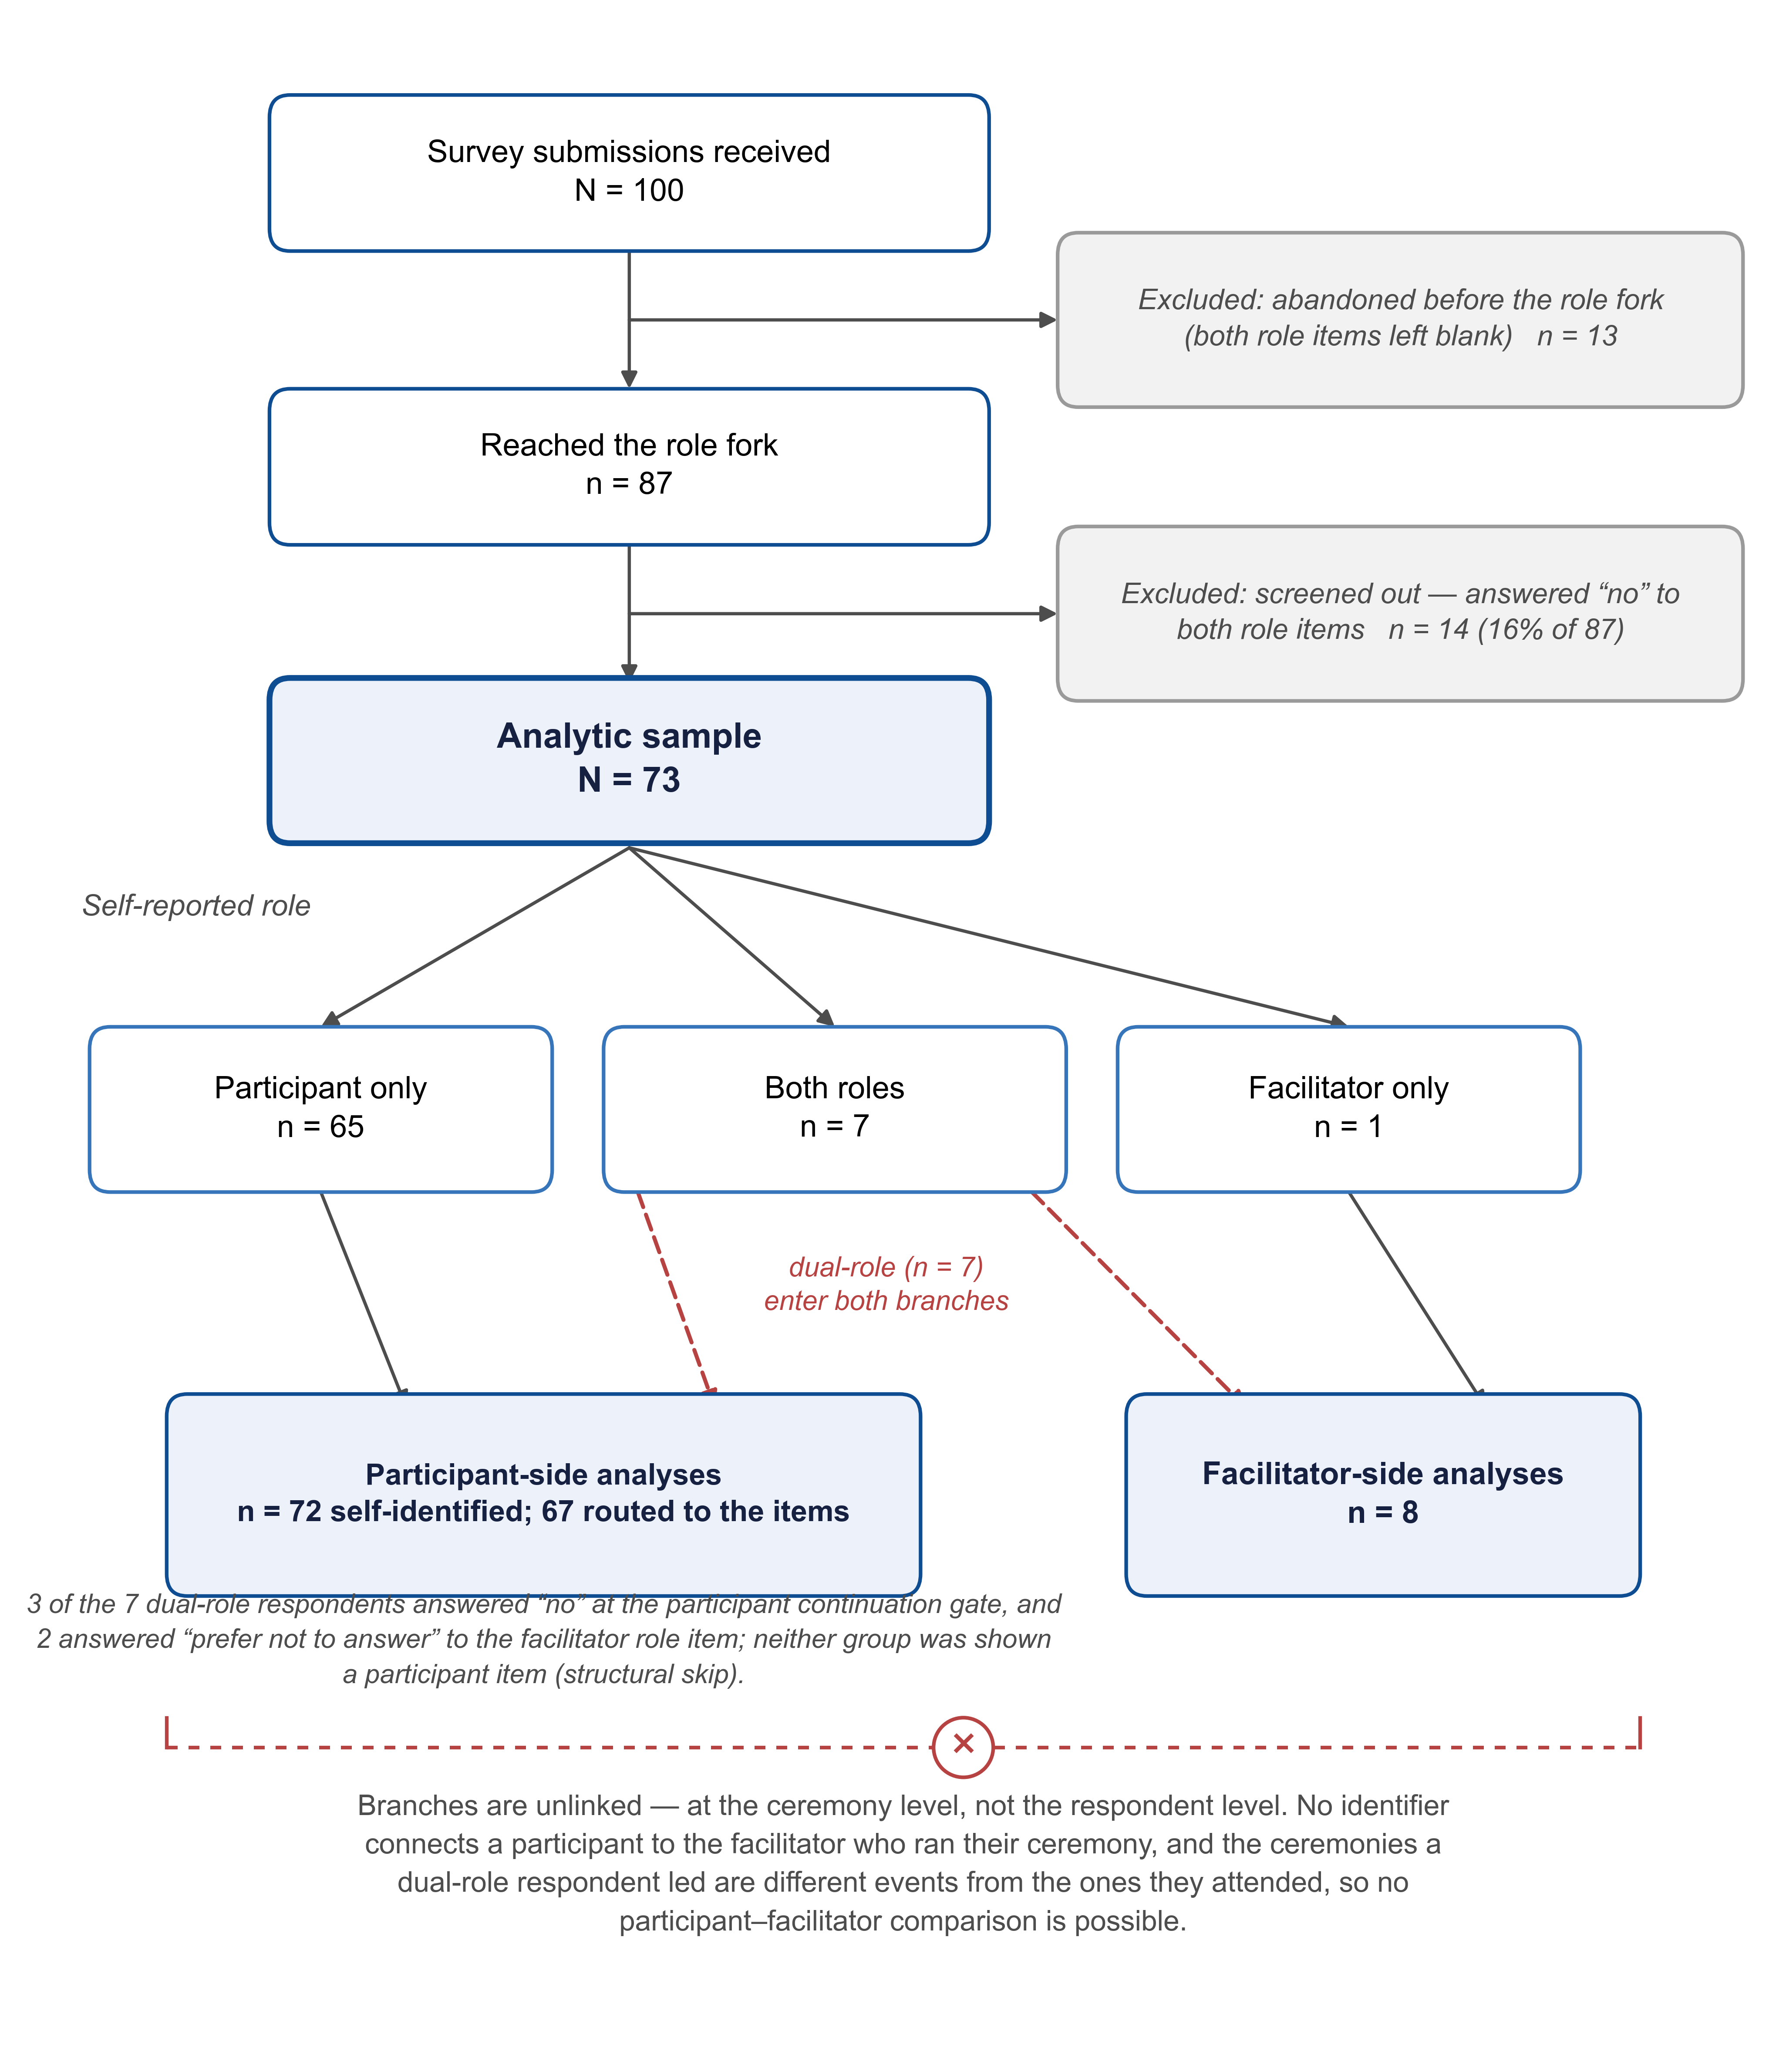
\includegraphics[width=0.94\textwidth]{../figures/fig1_flow.png}
\caption{Sample construction and role structure. Of 100 submissions, 13 were abandoned before the role
fork and 14 of the remaining 87 screened out by answering ``no'' to both role items, leaving an analytic
sample of $N=73$. Roles are not mutually exclusive: the 7 dual-role respondents enter both branches, giving
72 participant-side and 8 facilitator-side reports, and 3 of those 7 were stopped by the participant
continuation gate and 2 further participants answered ``prefer not to answer'' to the facilitator role item,
satisfying neither arm of the participant section's relevance condition, so 67 respondents were actually
routed to the participant items. The branches are unlinked at the ceremony level --- no identifier connects
a participant to the facilitator who ran their ceremony, and the ceremonies a dual-role respondent led are
different events from those they attended --- so no participant--facilitator comparison is possible.}
\label{fig:flow}
\end{figure}

\clearpage
\begin{figure}[htbp]
\centering
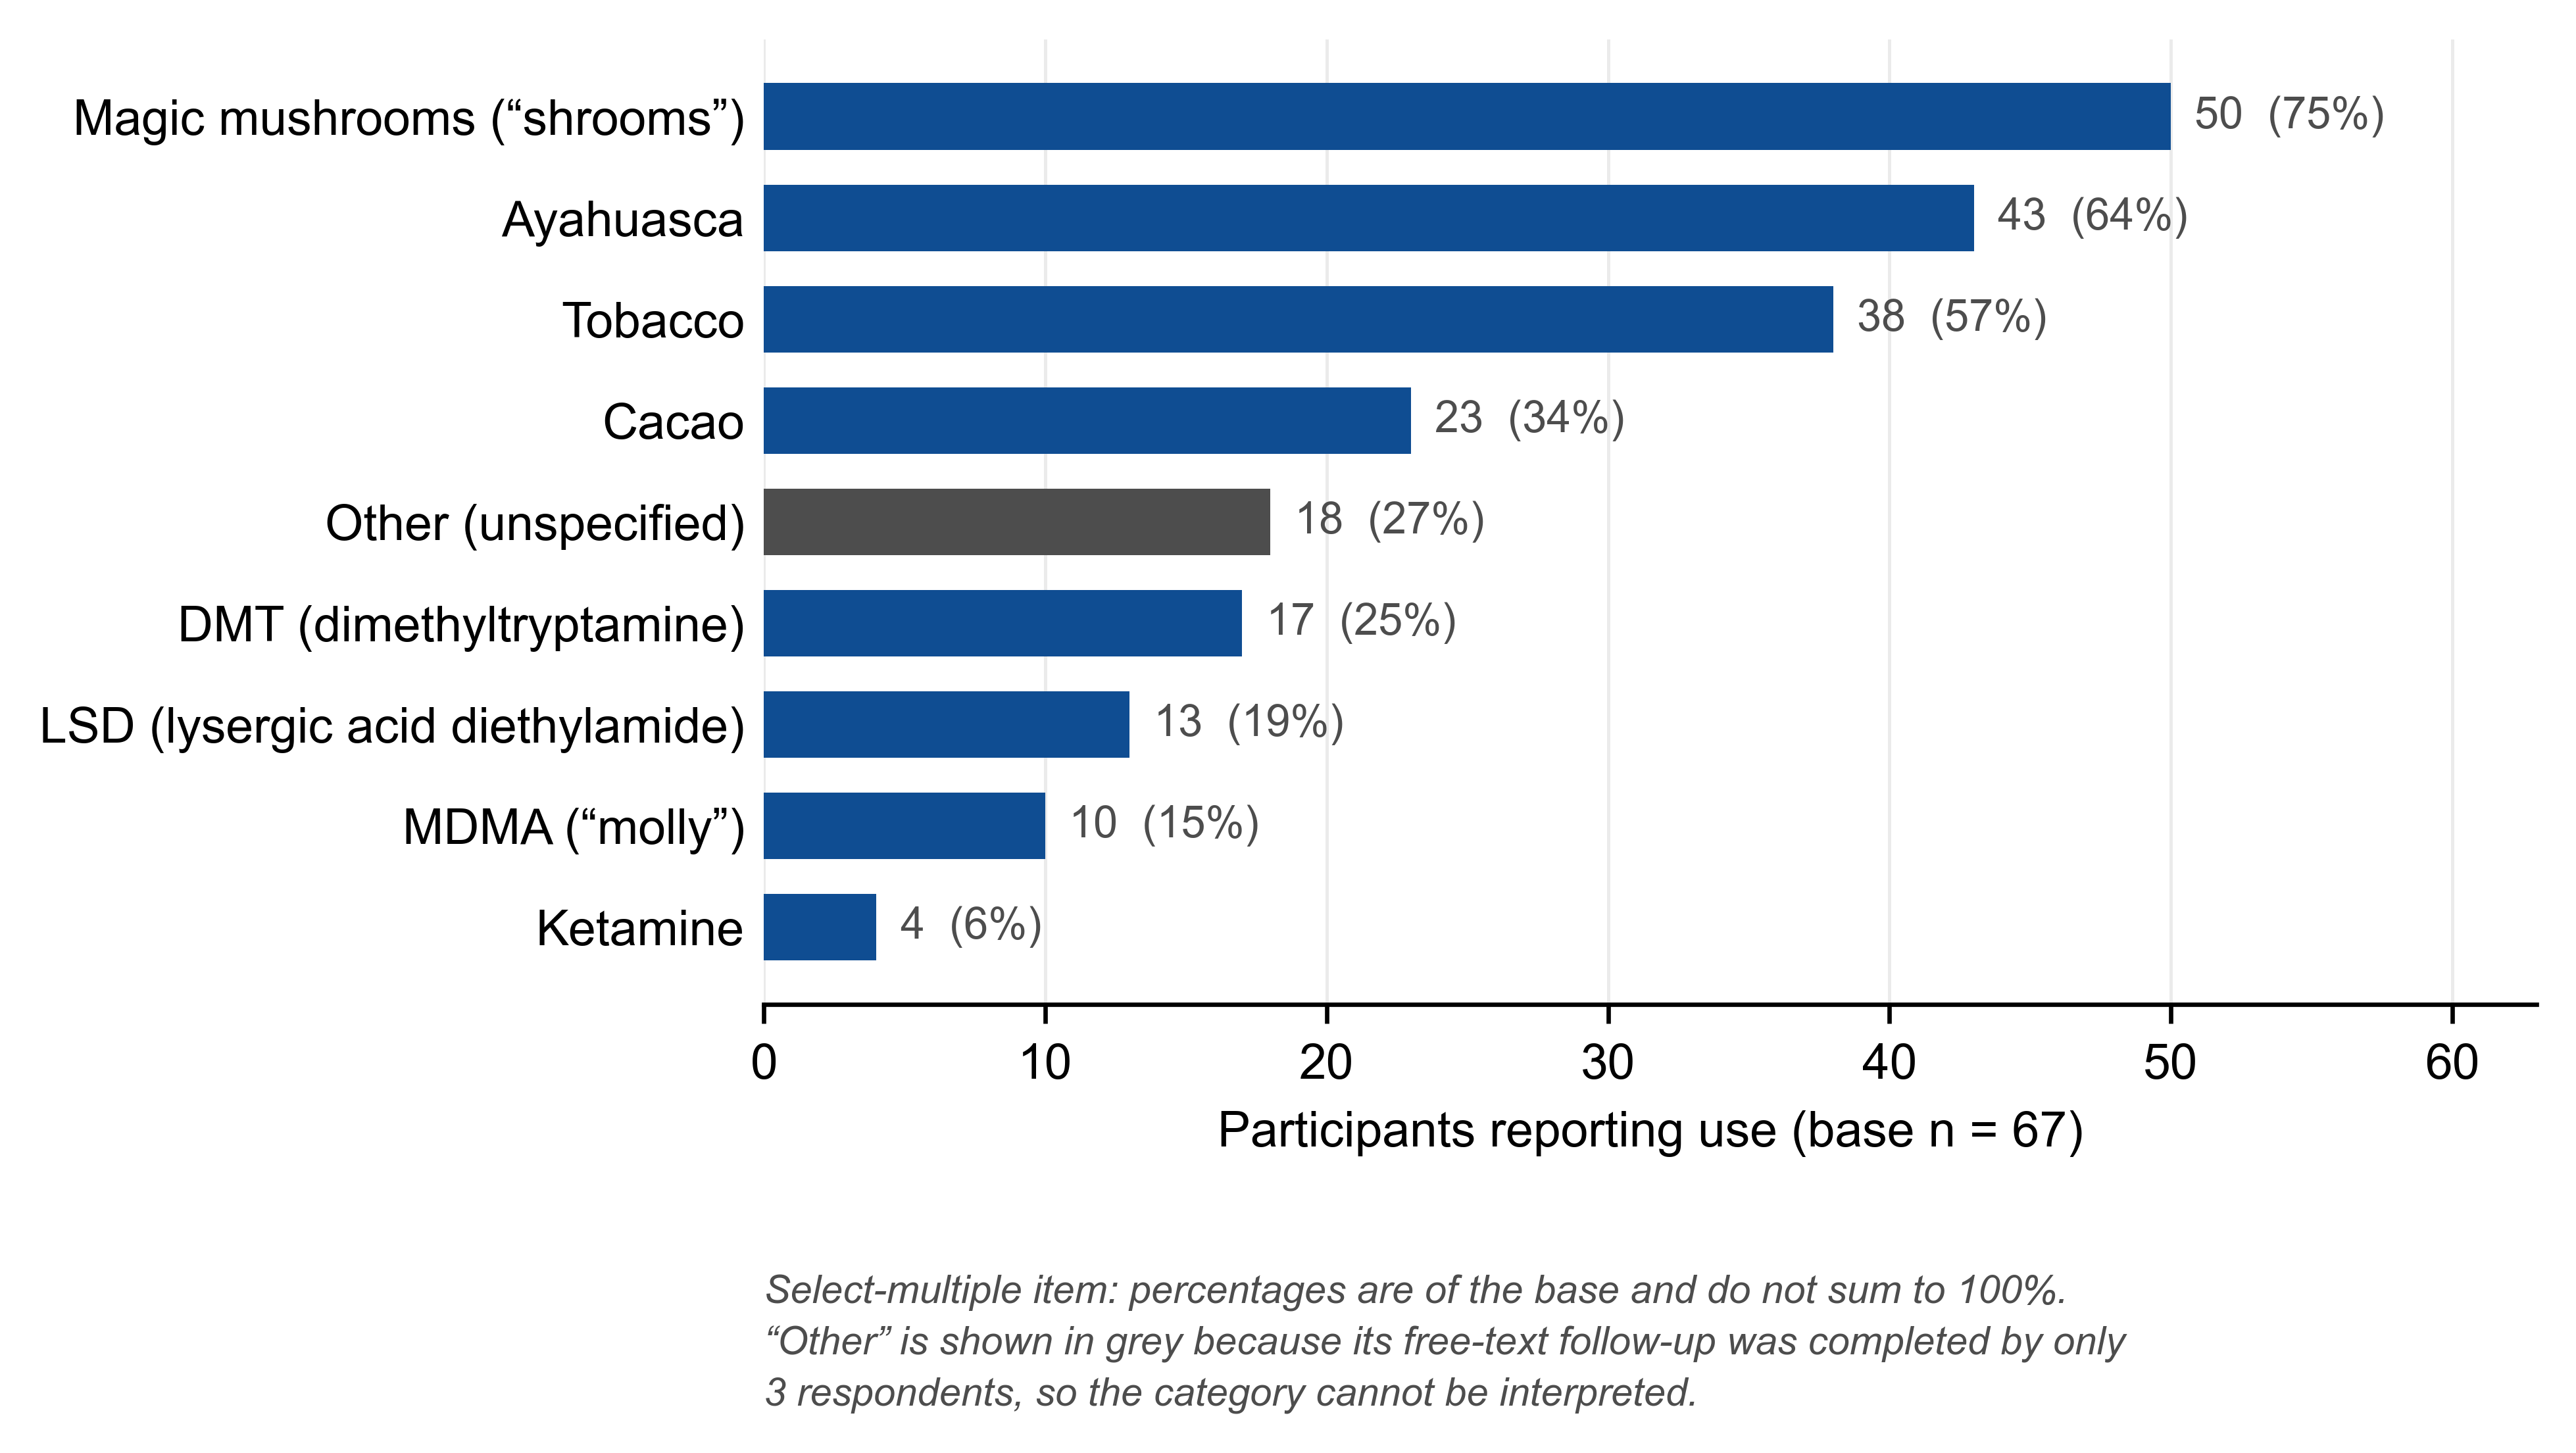
\includegraphics[width=\textwidth]{../figures/fig2_substances.png}
\caption{Substances used across all ceremonies attended, participant-reported (select-multiple; base $n=67$
participants answering). Bars are labeled with the count and the percentage of that base; because
respondents could select more than one substance, percentages need not sum to 100\%. The ``other'' bar is
drawn in grey because its free-text follow-up was completed by only 3 respondents. Distinct from the
facilitator-led substance variable and from the most-recent-ceremony substance variable.}
\label{fig:subs}
\end{figure}

\clearpage
\begin{figure}[htbp]
\centering
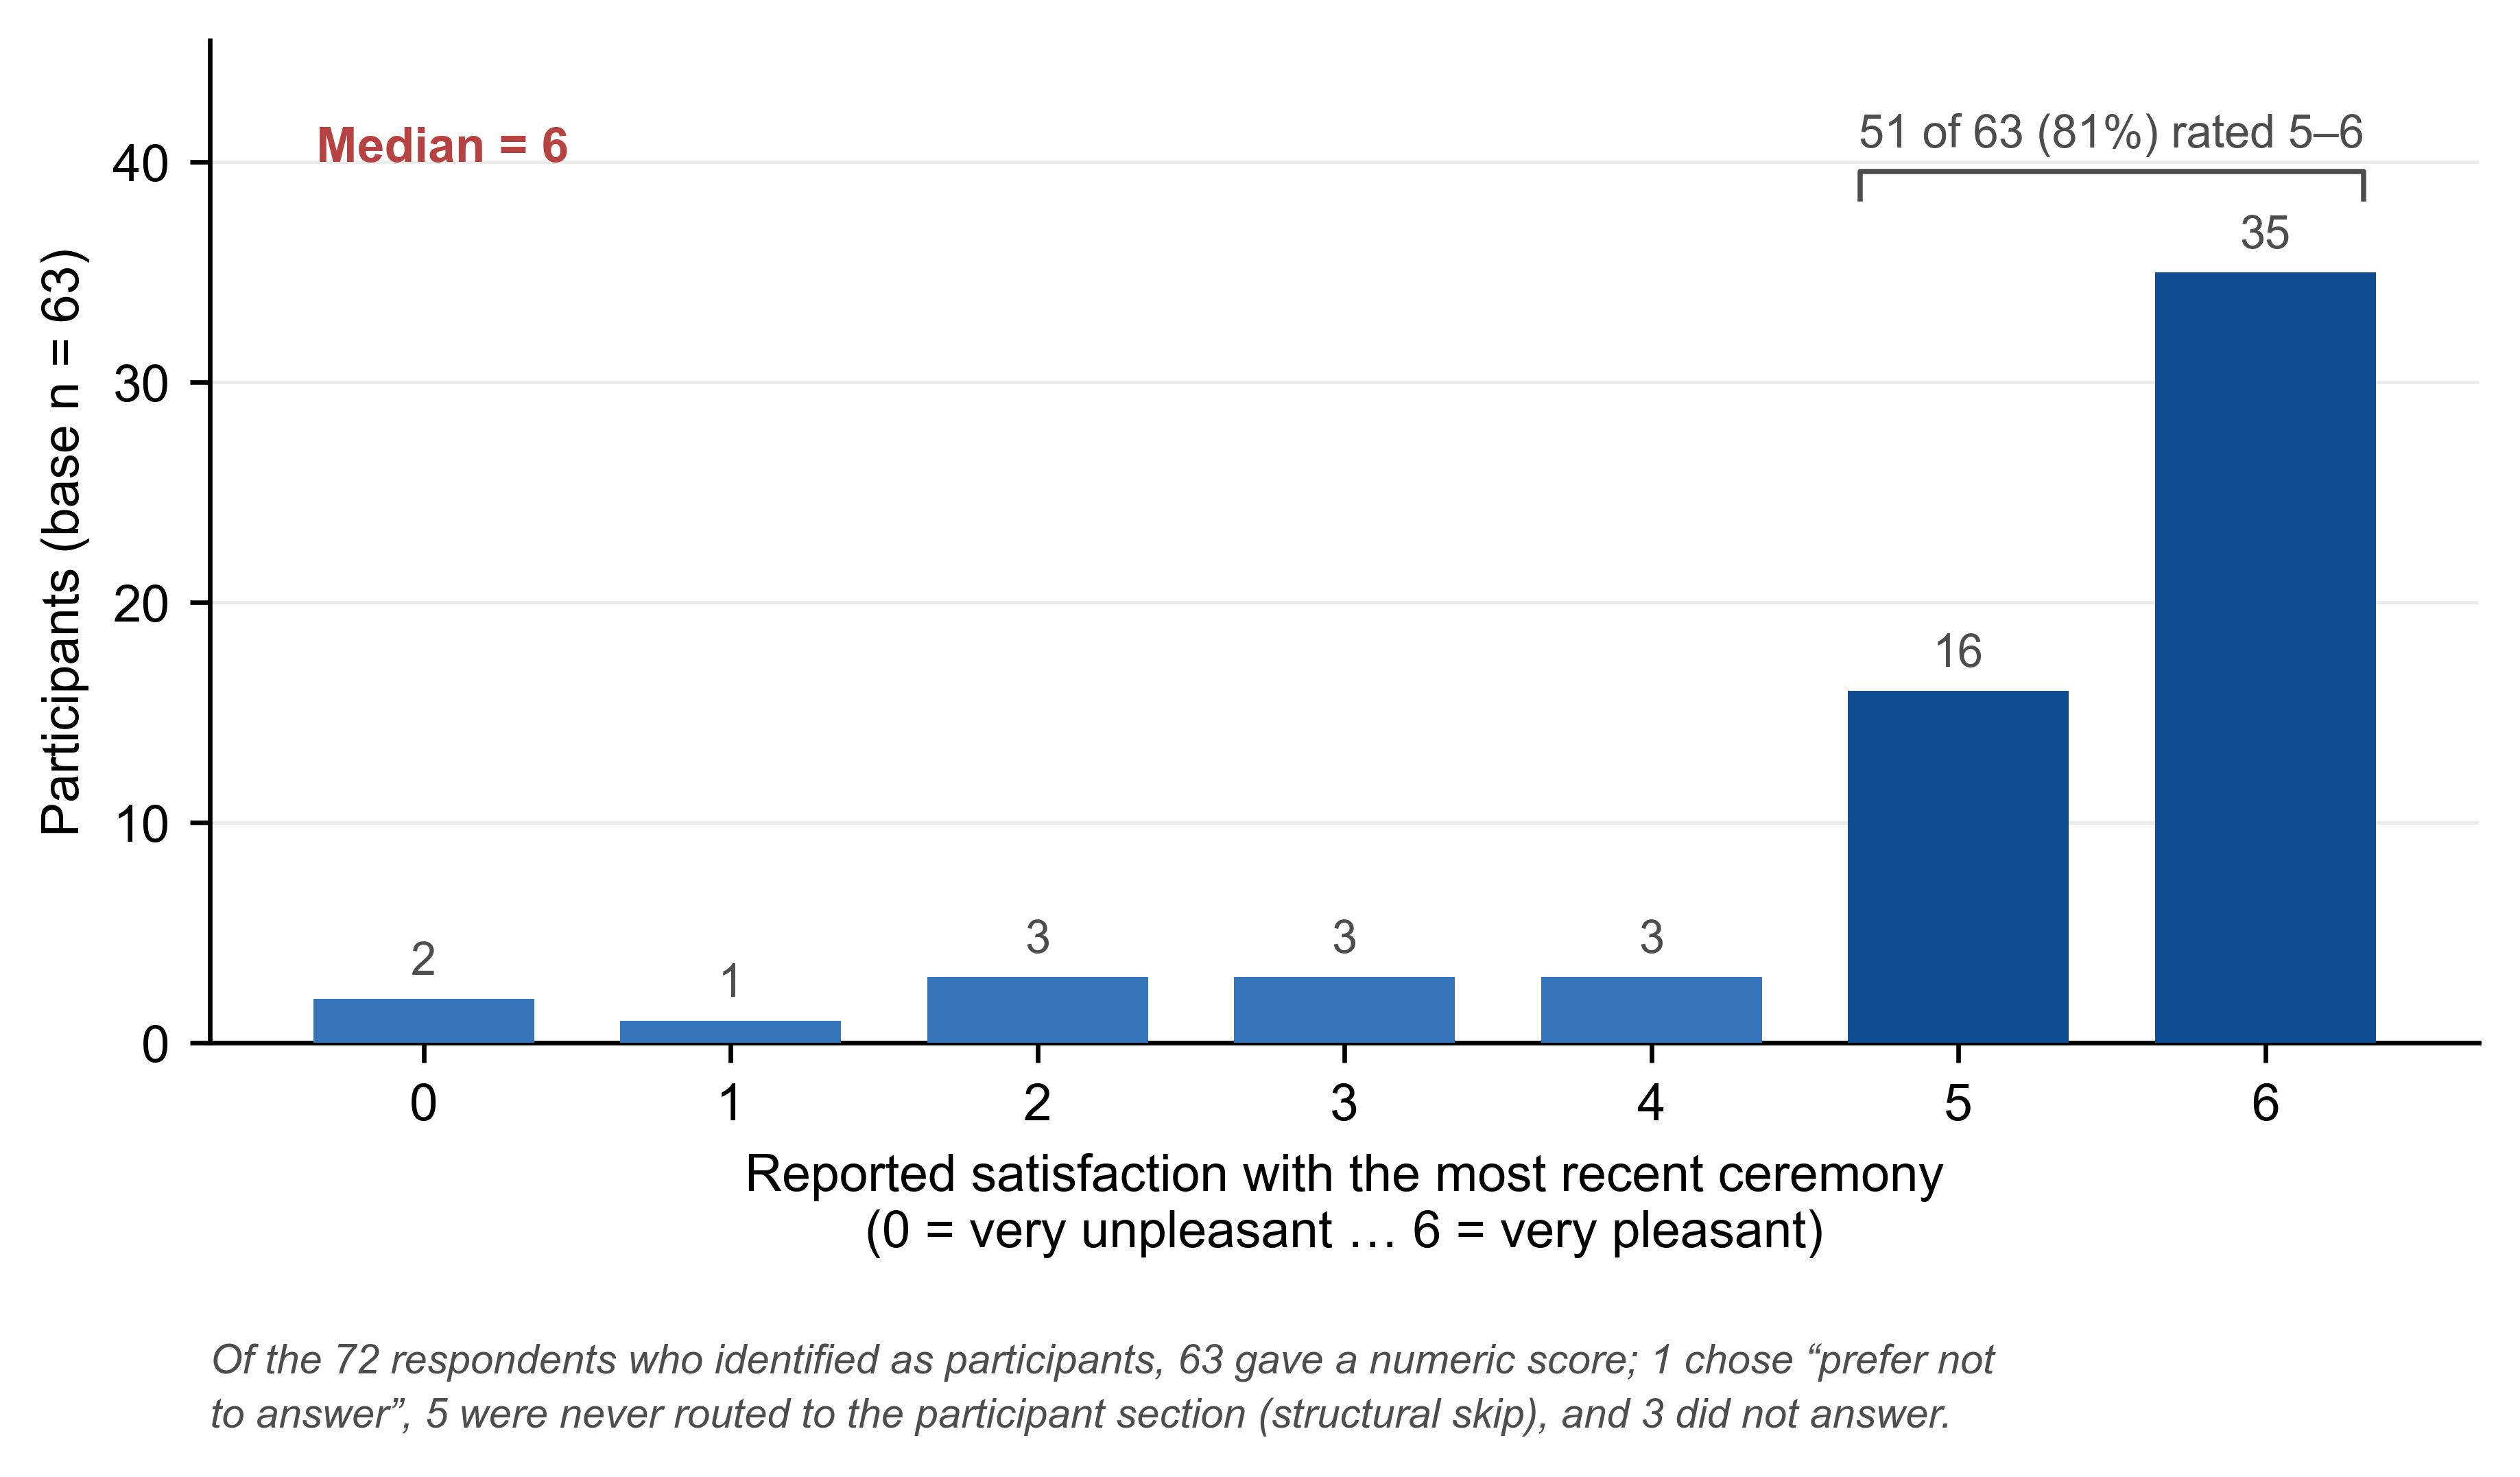
\includegraphics[width=\textwidth]{../figures/fig3_ceremony_good.png}
\caption{Distribution of reported satisfaction with the most recent ceremony (0 = very unpleasant to 6 =
very pleasant). Of the 72 respondents identifying as participants, 63 gave a numeric score and form the
base; the remaining 9 comprise 1 ``prefer not to answer'', 5 structural skips, and 3 item nonresponses.
Median 6, with 51 of 63 (81\%) answering 5 or 6 --- the ceiling that limits how much variance any predictor
can explain.}
\label{fig:good}
\end{figure}

\clearpage
\begin{figure}[htbp]
\centering
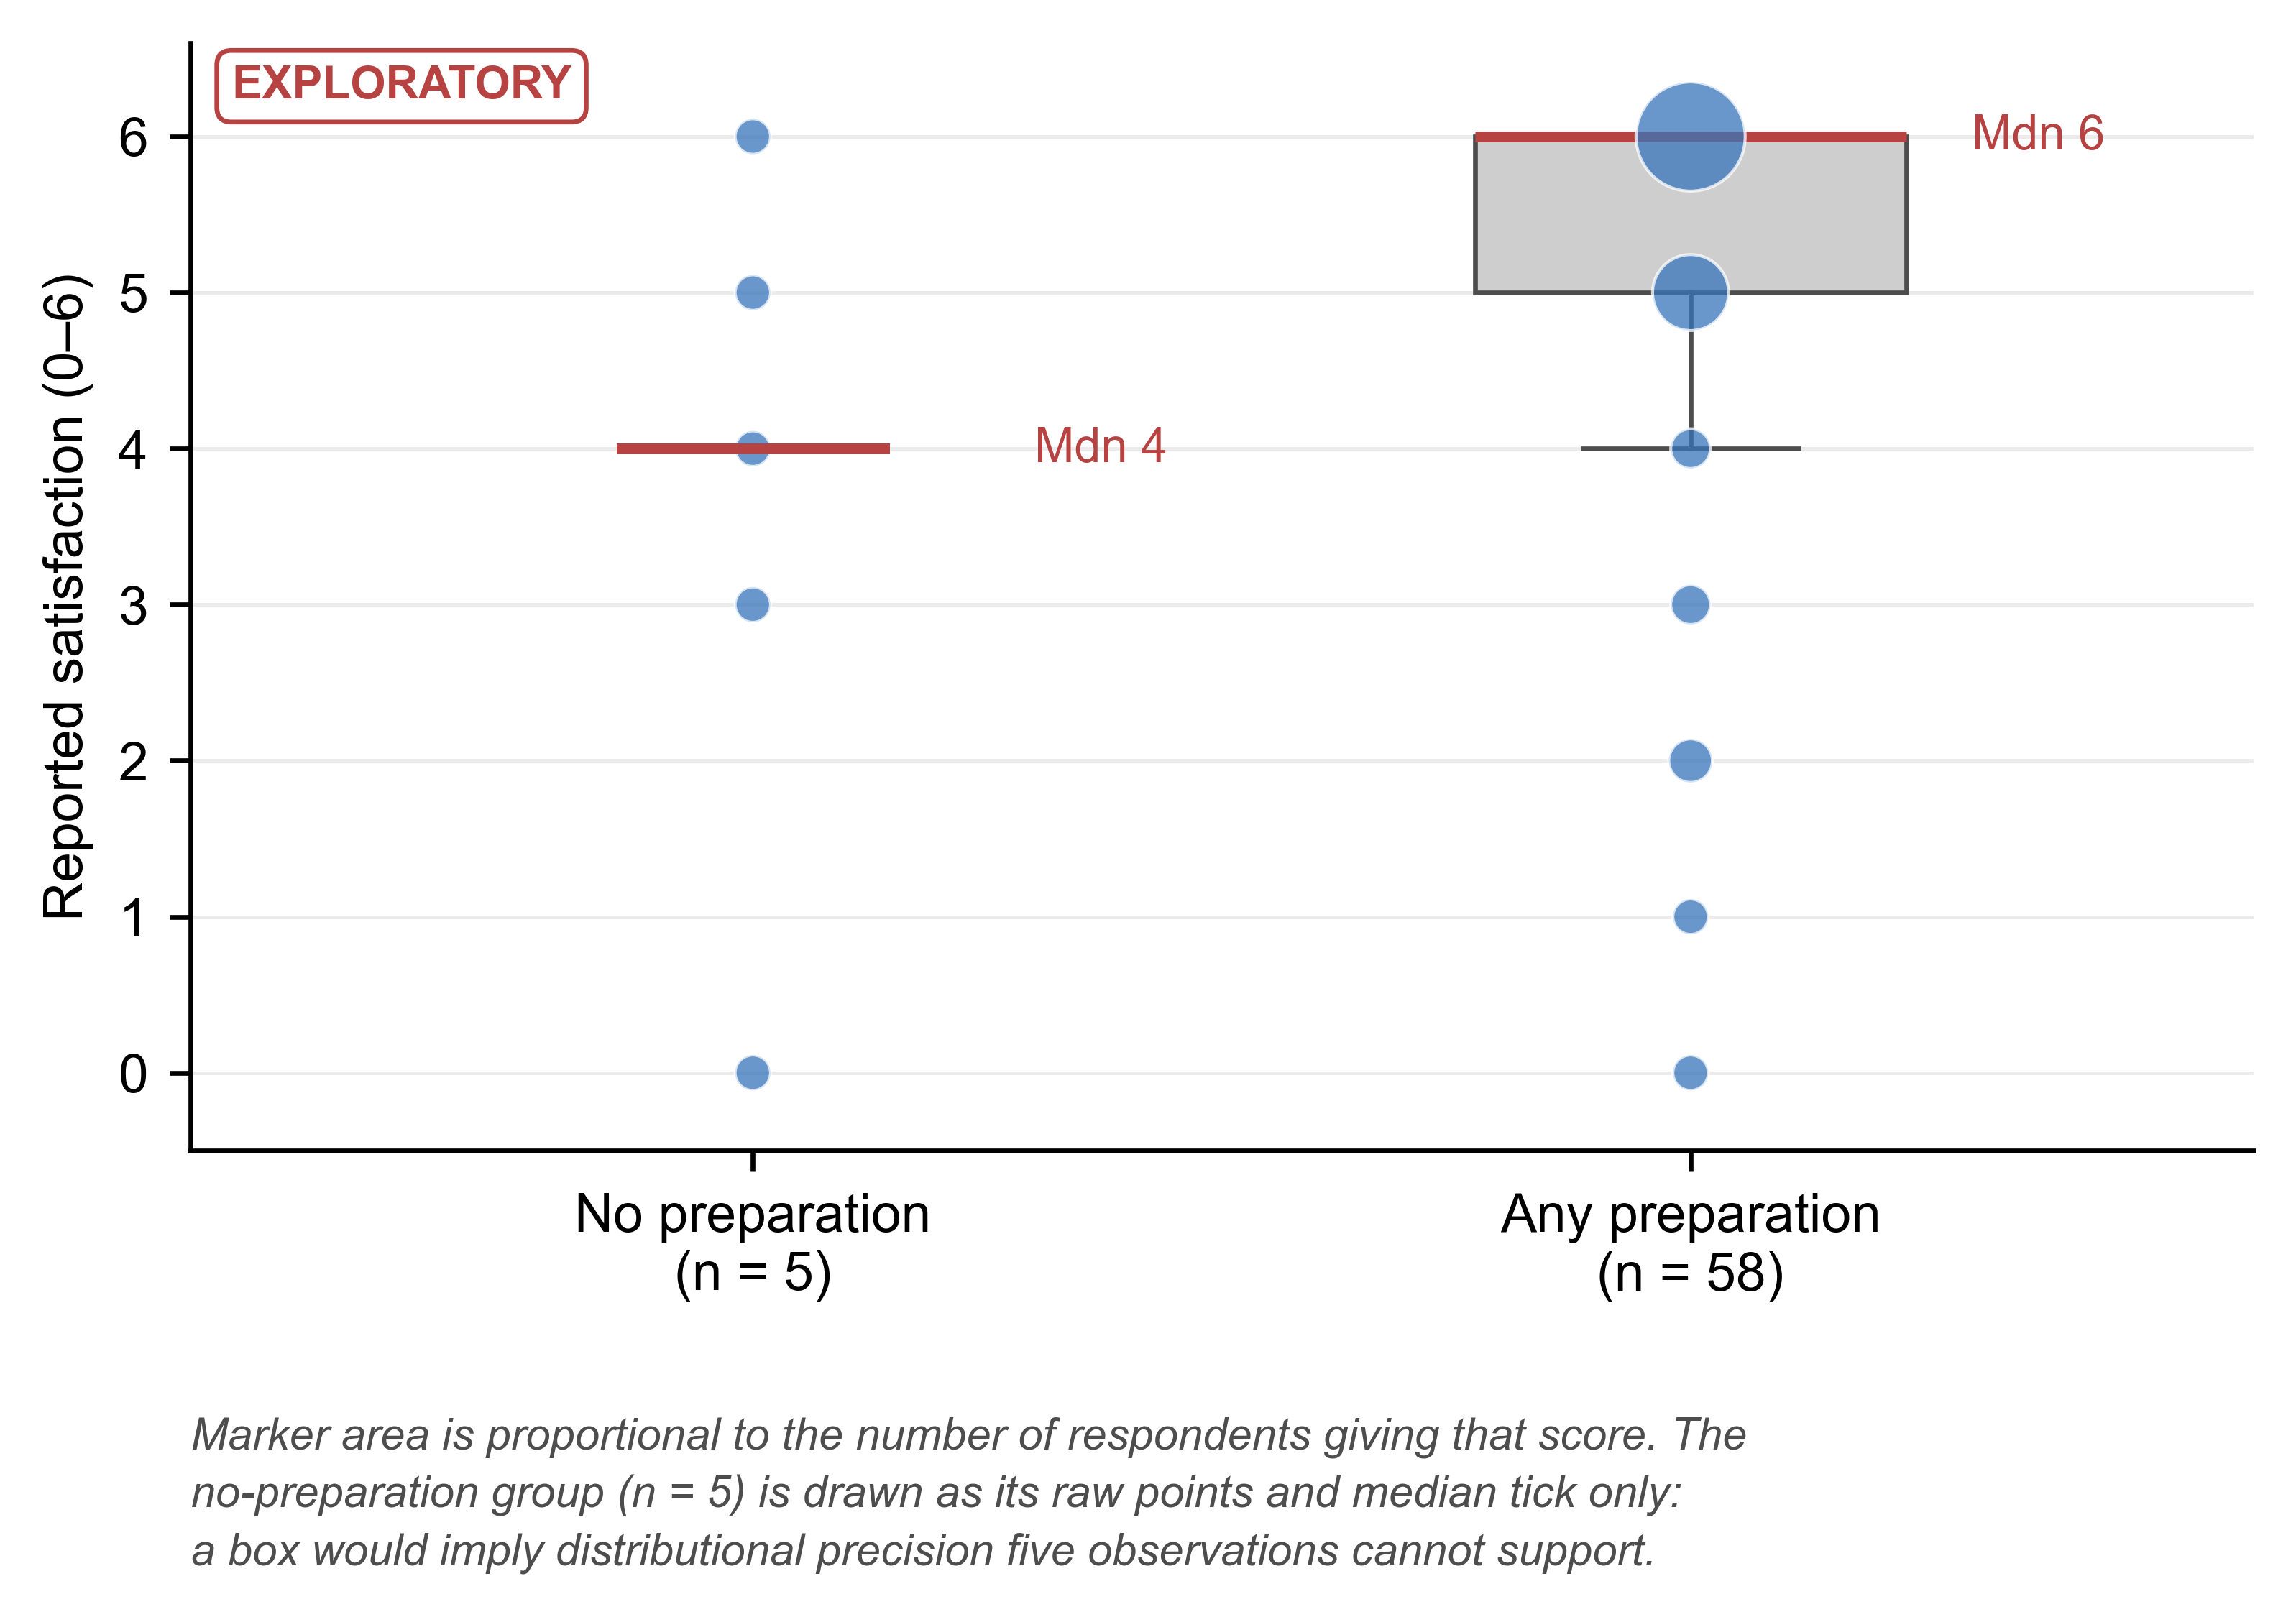
\includegraphics[width=\textwidth]{../figures/fig4_prep_outcome.png}
\caption{Reported satisfaction by self-directed preparation status. Any preparation, $n=58$ answering the
outcome (median 6, IQR 5--6); no preparation, $n=5$ (median 4, IQR 3--5). Marker area is proportional to the
number of respondents giving each score, since scores tie heavily at the ceiling. The no-preparation group
is drawn as its five raw points and a median tick rather than a box, which at that $n$ would imply
distributional precision the data cannot support. \textbf{Exploratory:} this comparison is suggestive, not
confirmatory.}
\label{fig:prep}
\end{figure}

\end{document}
